%\documentclass[11pt,a4paper]{article}
\usepackage[utf8]{inputenc}
\usepackage[dutch]{babel}
\usepackage{pgfplots}
\usepgfplotslibrary{units}
\usepackage{float}
\usepackage{amsmath,amsthm}
\usepackage{amsfonts}
\usepackage{amssymb}
\usepackage[left=2cm,right=2cm,top=2.5cm,bottom=2cm]{geometry}
\usepackage{graphicx}
\usepackage{multicol}
\usepackage{enumerate}
\usepackage{fancyhdr}
\pagestyle{fancy}
\usepackage{algorithm}
\usepackage{algpseudocode}
\usepackage{pgfplots}
\usepackage{multirow}
\usepackage{tikz}
\usetikzlibrary{calc}

\floatname{algorithm}{Algoritme}


\usepackage[font=small,labelfont=bf]{caption}
\captionsetup[table]{aboveskip=-0.8em}
\captionsetup[table]{belowskip=-0.7pt}


\lhead {DAIII Project: punten plaatsen} 
\chead{BAZ(~ \thepage ~ )NGA} 
\rhead{Robbert Gurdeep Singh}


\cfoot{} % get rid of the page number 

\usepackage{hyperref}
\usepackage{chngcntr}
\counterwithin*{section}{part}
\counterwithin{algorithm}{section}
\counterwithin{table}{section}
\counterwithin{figure}{section}

\hypersetup{
    colorlinks=false,
    pdfborder={0 0 0},
}

\author{Robbert Gurdeep Singh}
\title{{Project Algoritmen en datastructuren III}\\ \Huge Genetische algoritmen}
%\date{}



\pgfplotsset{compat=1.8}


\newcommand{\drawGraph}[4]{
\begin{tikzpicture}
\begin{axis}[scale only axis, 
	%x-as	
    xmin=0,
	xlabel=#1,	
	%y-as
	ylabel=#2,
	ymin=0,
	%Style
	height=5em,width=.37\textwidth,
	enlargelimits=0.05,
	grid=major,	legend pos=south east
]
#3
\end{axis}
\end{tikzpicture}
}


\newcommand{\lxaxis}[3]{\begin{tikzpicture}
\begin{axis}[scale only axis, 
cycle list name=exotic,
    xmode=log,
    log ticks with fixed point,
	%x-as	
	xlabel=#2,	
	%y-as
	ylabel=#1,
	ymin=0,
	%Style
	height=5em,width=.37\textwidth,
	enlargelimits=0.05,
	grid=major,	legend pos=south east
]
#3

\end{axis}
\end{tikzpicture}}

\newcommand{\rlxaxis}[3]{\begin{tikzpicture}
\begin{axis}[scale only axis, 
cycle list name=exotic,
    xmode=log,
    log ticks with fixed point,
	%x-as	
	xlabel=#2,	
	%y-as
	ylabel=#1,
	%Style
	height=5em,width=.37\textwidth,
	enlargelimits=0.05,
	grid=major,	legend pos=south east
]
#3

\end{axis}
\end{tikzpicture}}

\newcommand{\nxaxis}[3]{\begin{tikzpicture}
\begin{axis}[scale only axis,
cycle list name=exotic, 
	%x-as	
    xmin=0,
	xlabel=#2,	
	%y-as
	ylabel=#1,
	ymin=0,
	%Style
	height=5em,width=.37\textwidth,
	enlargelimits=0.05,
	grid=major,	legend pos=south east
]
#3

\end{axis}
\end{tikzpicture}}


\newcommand{\rnxaxis}[3]{\begin{tikzpicture}
\begin{axis}[scale only axis, 
cycle list name=exotic,
	%x-as	
    xmin=0,
	xlabel=#2,	
	%y-as
	ylabel=#1,
	%Style
	height=5em,width=.37\textwidth,
	enlargelimits=0.05,
	grid=major,	legend pos=south east
]
#3

\end{axis}
\end{tikzpicture}}

\newcommand{\itemMB}[1]{
	\item[$\boldsymbol{#1}$:]
}




\newcommand{\abs}[1]{
	\lvert #1 \rvert
}

\newcommand{\addploti}[1]{\addplot table [y=i, x=testValue, col sep=comma] {../../tests/param_results/#1.log};}
\newcommand{\addplotf}[1]{\addplot table [y=f, x=testValue, col sep=comma] {../../tests/param_results/#1.log};}
\newcommand{\addplott}[1]{\addplot table [y=t, x=testValue, col sep=comma] {../../tests/param_results/#1.log};}

\definecolor{mymark}{HTML}{EBB8B8}

\begin{document}

\twocolumn[\begin{@twocolumnfalse}
    \maketitle
\end{@twocolumnfalse}]

\section{Toelichting Code}
In deze sectie gaan we wat dieper in op enkele programeerkeuzes
die niet tot het algoritmische horen, maar die we wel graag vermelden.
\label{sec:explainationcode}
\subsection{Gebruik heap}
\label{sub:heap}
\begin{figure}[H]
\centering
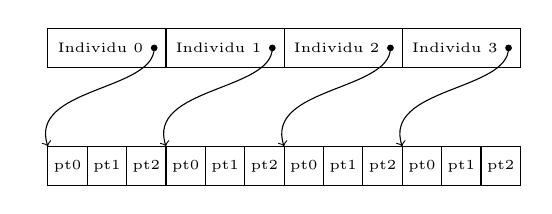
\begin{tikzpicture}
\foreach \x in {0,1,2,3}{
    \draw (1.5*\x,5) rectangle node {\tiny Individu \x~~~} (1.5*\x+1.5,4.5);
    
	\draw[->] (1.5*\x+1.35,4.75) .. controls (1.5*\x+1.35,4.2) and (1.5*\x-0.25,4.25) .. (1.5*\x,3.5);
	\draw[fill=black] (1.5*\x+1.35,4.75) circle (1pt);
	\foreach \y in {0,1,2}
    	\draw (1.5*\x+0.5*\y,3) rectangle node {\tiny pt\y} (1.5*\x+0.5*\y+0.5,3.5);
}

\end{tikzpicture}
\caption{De individu array en de punten array op de heap}
\end{figure}
Om de individuen bij te houden hebben we er voor gekozen ze in 1 lange rij op de heap te plaatsen. Dit zorgt ervoor dat we de populatiegrootte at runtime kunnen bepalen, wat handig kan zijn bij de parallelle  uitvoering. We houden ook 1 lange array van punten bij op de heap. Deze array bevat $n\cdot N_p$ punten. Elk van de individuen heeft een pointer die naar een plaats in deze array wijst. Het in één keer alloceren zorgt ervoor dat we tijdens de uitvoering geen overhead hebben door allocaties. Het zorgt er ook voor dat we minder gemakkelijk memory leaks enzo hebben.

\subsection{Plaats kideren}
Na het paren zijn er meer individuen in de populatie. Om deze een plaats in het geheugen te geven maken tijdens de initialisatie de arrays waarin we het in Sectie~\ref{sub:heap} hadden extra ``lege'' plaatsen. De kinderen worden dan gestokeerd vanaf index $N_p$.

Door deze grotere array te nemen wordt het ook gemakelijker om tournament selection to te passen op heel de populatie.

\subsection{Tests}
\label{sub:explain_tests}
Om te testen of bepaalde stukken code wel werkten hebben we testen geschreven. Deze zijn te vinden in \texttt{main.c} en kunnen worden geactiveerd met de \texttt{-D} vlag van de compiler.

\subsection{Debuging}
\label{sub:explain_debug_analyse}
Tijdens de ontwikkeling wilden we graag zien hoe de fitheid verliep in de tijd. Hiervoor hebben we een \texttt{log\_dbg} macro geintroduceerd die enkel print als er gecompileerd werdt met \texttt{-DDEBUG}.

Om de performantie gemakkelijk te testen met Python hebben we een {\em{Performance Print}} mode toegevoegd. Deze wordt geactiveerd door te compilen met  \texttt{-DPERFORMANCE\_PRINT}. In deze mode wordt enkel het aantal iteraties en de bekomen fitheid geprint.

% subsection  (end)
% section explainationcode (end)

%\section{Bronnen}
Er moet vermeld worden dat het \texttt{icosagon.poly} bestand afkomstig is van Jonathan Peck. We hebben dit bestand uitgewisseld om een andere figuur dan het gegeven vierkant te hebben samen met een notie van de maximale fitheid voor 50 punten in deze figuur. Code is er natuurlijk niet uitgewisseld.

\begin{thebibliography}{9}

\bibitem{lamport94}
  Haupt, Randy L., and Sue Ellen Haupt. ``Practical genetic algorithms.'' (2004).

\bibitem{baker85}
Baker, James Edward. "Adaptive selection methods for genetic algorithms." Proceedings of an International Conference on Genetic Algorithms and their applications. 1985.

\bibitem{parra9748125}
Pit, Laurens Jan. "Parallel genetic algorithms." MS (Computer Sci.) Dissertation (1995).

\bibitem{cuofiezafm}
Brinkmann, Gunnar. "Datastructuren en Algoritmen III, 2014." Cursus (2014)

\bibitem{MPIDOC}
University of Tennessee, "MPI: A Message-Passing Interface Standard" Online PDF. http://www.mpi-forum.org/docs/mpi-3.0/mpi30-report.pdf (2012)



\end{thebibliography}
\end{document}